\documentclass[9pt,twocolumn,twoside,]{pnas-new}

% Use the lineno option to display guide line numbers if required.
% Note that the use of elements such as single-column equations
% may affect the guide line number alignment.


\usepackage[T1]{fontenc}
\usepackage[utf8]{inputenc}

% tightlist command for lists without linebreak
\providecommand{\tightlist}{%
  \setlength{\itemsep}{0pt}\setlength{\parskip}{0pt}}


% Pandoc citation processing
\newlength{\cslhangindent}
\setlength{\cslhangindent}{1.5em}
\newlength{\csllabelwidth}
\setlength{\csllabelwidth}{3em}
\newlength{\cslentryspacingunit} % times entry-spacing
\setlength{\cslentryspacingunit}{\parskip}
% for Pandoc 2.8 to 2.10.1
\newenvironment{cslreferences}%
  {}%
  {\par}
% For Pandoc 2.11+
\newenvironment{CSLReferences}[2] % #1 hanging-ident, #2 entry spacing
 {% don't indent paragraphs
  \setlength{\parindent}{0pt}
  % turn on hanging indent if param 1 is 1
  \ifodd #1
  \let\oldpar\par
  \def\par{\hangindent=\cslhangindent\oldpar}
  \fi
  % set entry spacing
  \setlength{\parskip}{#2\cslentryspacingunit}
 }%
 {}
\usepackage{calc}
\newcommand{\CSLBlock}[1]{#1\hfill\break}
\newcommand{\CSLLeftMargin}[1]{\parbox[t]{\csllabelwidth}{#1}}
\newcommand{\CSLRightInline}[1]{\parbox[t]{\linewidth - \csllabelwidth}{#1}\break}
\newcommand{\CSLIndent}[1]{\hspace{\cslhangindent}#1}


\templatetype{pnasresearcharticle}  % Choose template

\title{Diversité des collaborations des élèves du cours BIO500 à l'hiver
2022}

\author[a]{Marguerite Duchesne}
\author[a]{Florian Jordan}
\author[a]{Anthony St-Pierre}
\author[a]{Simon Grégoire}
\author[a]{Francis Lessard}

  \affil[a]{Université de Sherbrooke, Départment de biologie, 2500
Boulevard de l'Université, Sherbrooke, Québec, J1K 2R1}


% Please give the surname of the lead author for the running footer
\leadauthor{}

% Please add here a significance statement to explain the relevance of your work
\significancestatement{}


\authorcontributions{}



\correspondingauthor{\textsuperscript{} }

% Keywords are not mandatory, but authors are strongly encouraged to provide them. If provided, please include two to five keywords, separated by the pipe symbol, e.g:
 \keywords{  Collaborations |  Réseau écologique |  Travaux d'équipe  } 

\begin{abstract}
Nous avons voulu nous intérésser aux collaborations des élèves de
l'Université de Sherbrooke lors de travaux d'équipe pendant leur
parcours dans le baccalauréat en biologie. Pour ce faire, nous avons
dressé un réseau reliant tous les étudiants qui ont suivi le cours de
méthodes en écologie computationnelle (BIO500) lors de la session
d'hiver 2022 et qui démontre le nombre de collaborations qui ont eu lieu
entre eux tout au long de leur parcours universitaire. Nous avons
comparé le nombre total de collaborations de chaque étudiant ainsi que
le nombre de collaborations différentes de chaque étudiant dans le but
de déterminer s'ils ont tendance à conserver les mêmes équipes ou non.
Nous avons aussi observé l'impact que le cours de méthodes analytiques
en biologie (TSB303) possédait sur le réseau puisque ce dernier comporte
un travail d'équipe de 15 personnes. Nous avions un soupçon qu'un
travail de cette ampleur modifierait beaucoup le réseau final, et à la
lumière de nos résultats, cette hypothèse a été confirmée. On peut aussi
facilement identifier sur le réseau les groupes de travail qui se sont
maintenus à travers le baccalauréat, ce qui prouve que les étudiants
n'avaient pas tendance à beaucoup diversifier leurs collaborations.
\end{abstract}

\dates{This manuscript was compiled on \today}
\doi{\url{www.pnas.org/cgi/doi/10.1073/pnas.XXXXXXXXXX}}

\begin{document}

% Optional adjustment to line up main text (after abstract) of first page with line numbers, when using both lineno and twocolumn options.
% You should only change this length when you've finalised the article contents.
\verticaladjustment{-2pt}



\maketitle
\thispagestyle{firststyle}
\ifthenelse{\boolean{shortarticle}}{\ifthenelse{\boolean{singlecolumn}}{\abscontentformatted}{\abscontent}}{}

% If your first paragraph (i.e. with the \dropcap) contains a list environment (quote, quotation, theorem, definition, enumerate, itemize...), the line after the list may have some extra indentation. If this is the case, add \parshape=0 to the end of the list environment.

\acknow{}

\hypertarget{introduction}{%
\section{Introduction}\label{introduction}}

On entend souvent l'expression « Ah que le monde est petit ! » lorsque
deux personnes se retrouvent à avoir une connexion qu'on ne suspectait
pas. Certaines études se sont intéressées à ce principe selon lequel
tout le monde est lié à un certain niveau. Milgram (1967) s'est penché
sur le sujet et à testé cette hypothèse selon laquelle deux personnes
pigées au hasard devraient avoir un lien rapproché entre eux (1). Ce
principe peut également s'appliquer à l'écologie, au niveau de vu de
l'évolution, toutes les espèces sont reliées par un ancêtre commun (2).
Les réseaux trophiques présentent aussi ce genre de dynamique (2). Ce
modèle de « petit monde » peut donc s'appliquer à grande et petite
échelle. Nous avons voulu observer cette théorie à très petite échelle
dans le baccalauréat de la 59e cohorte d'écologie de l'Université de
Sherbrooke. L'école forme les futurs travailleurs de demain, et avoir un
grand nombre de collaborations à l'université peut être bénéfique si on
se fie aux recommandations de plusieurs firmes aidant les travailleurs à
optimiser leurs capacités au travail. Un réseau de collaborations
diversifié entraîne un engagement plus élevé des employés, une meilleure
rétention et plus d'innovation (Holtzman and Anderberg, 2011). Nous nous
sommes donc posés la question si le réseau de collaborations entre les
étudiants du baccalauréat en écologie favorisait la diversité des
collaborations. Plus spécifiquement, nous avons étudié si les élèves
ayant une grand nombre de collaborations ont davantage tendance à
diversifier leurs partenaires. En effet, il est intéressant de voir si
les étudiants ont plusieurs groupes de collaborateurs ou si, au cours du
baccalauréat, ils ont entretenus des liens avec les mêmes personnes.
Pour les gens pour lesquels on juge avoir un grand nombre de
collaborations, est-ce qu'il y a un moyen de trouver ce qui leur a
permis d'obtenir ce nombre de collaborations? Nous avons également
vérifié si le cours de méthodes analytiques en biologie (TSB303) a eu un
grand effet dans le réseau de collaborations, puisque dans ce cours, le
travail était pour la plupart en équipe de 9. On peut donc s'imaginer
qu'à lui seul, ce cours ajoute beaucoup de collaborations entre les
étudiants. Le réseau de collaboration entre les étudiants ayant plus de
30 collaborations sera aussi produit pour observer si la dynamique des
liens entre étudiant change dans cette situation. Pour aider à
visualiser le tout, une première figure va détailler toutes les
collaborations entre tous les individus de la cohorte. Puis, plus
spécifiquement, une autre figure mettra en évidence les collaborations
du cours TSB303. Ensuite, Un réseau plus petit fesant l'emphase sur les
étudiant ayant un grand nombre de collaborations sera illustré.

\hypertarget{muxe9thode}{%
\section{Méthode}\label{muxe9thode}}

La classe de BIO500 de la session d'hiver 2022 s'est divisée en 9
équipes. Chaque élève de ces équipes a compilé l'ensemble des cours pour
lesquel des travaux d'équipe ont été réalisés lors de son baccalauréat.
Ces information ainsi que l'informations considérées pertinentes reliées
à ces cours dans une première table commune à l'équipe. Ils ont
également compilé dans une seconde table le nom de chaque coéquipier
ainsi que de leurs collaborateurs. Pour chacun des étudiant, l'année de
début de leur baccalauréat, le nom de leur programme et leur
participation au régime coopératif à été ajoutés. Ils ont terminé la
compilation des données par une troisième table. Au sein de cette
dernière table se trouve l'ensemble des collaborations, c'est-à-dire
leurs liens collaboratifs avec d'autre étudiant et le travail d'équipe
correspondant à ce lien.

Une fois la compilation des données réalisée par chaque équipe, celle-ci
fut partagée et mise en commun. Maintenant indépendantes, les équipes
avaient alors la tâche de fusionner l'ensemble des données afin d'avoir
que trois tables contenant l'ensemble des données de la classe, ceci a
été effectué dans le logiciel R. Au préalable, chaque équipe a dû
standardiser les données de l'ensemble des équipes afin d'obtenir une
conformité au sein des différentes tables. Ces données ont ensuite été
injectées dans le système de gestion de données SQLite3. Afin de
répondre à la question posée, les données d'intérêt ont été extraites
via des requêtes et analysées. Les représentations visuelles des réseau
ont été effectué grâce au package Igraph du locigiel R. Finalement, le
package targets a été utilisé afin d'automatisé l'ensemble du processus
et d'augmenter la reproductibilité de la démarche.

\hypertarget{ruxe9sultats}{%
\section{Résultats}\label{ruxe9sultats}}

Pour mieux illustrer les réponses aux questions, plusieurs figures
présenteront les liens entre les étudiants.

\begin{figure}
\centering
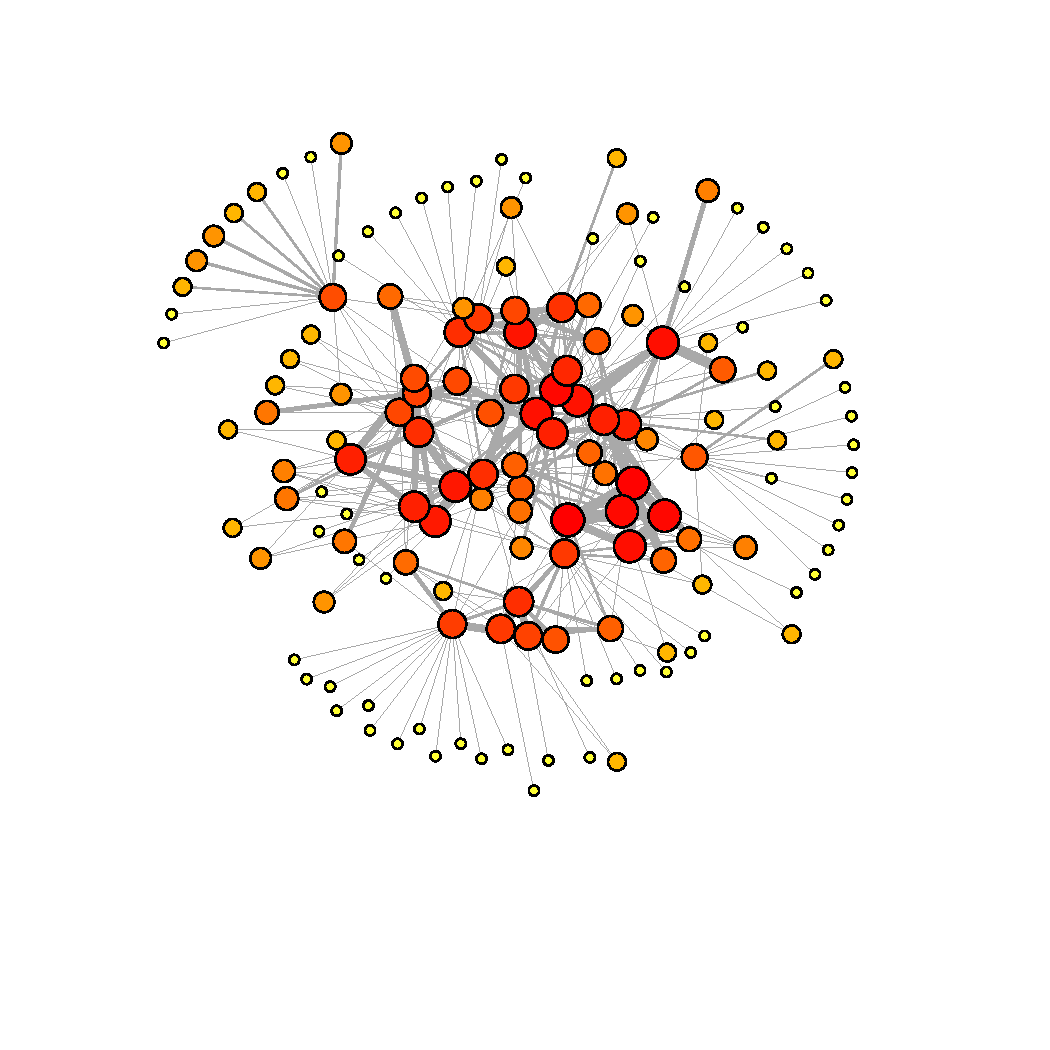
\includegraphics[width=0.5\textwidth,height=0.4\textheight]{"../results/figure1.png"}
\caption{Réseau de collaboration des étudiants de la du cours BIO500
l'hiver 2022.La grandeur et la couleurs des noeuds sont déterminées par
une comparaison relative du nombre collaborations de chaque élève, les
cercles les plus petits et jaunes correspondant à une seule
collaboration.La largeur des liens correspond au nombre de
collaborations entre la paire d'étudiant. \label{fig:plot1}}
\end{figure}

La figure \ref{fig:plot1} représente le réseau de toutes les
collaborations des étudiants du cours de méthodes en écologie
computationnelle (BIO500) à l'hiver 2022. Dans cette siutation, La
moyenne de liens par étudiant est de 10.67, la distance maximale entre
deux étudiant est de 5 liens et la modularité du réseau est de 0.635.

La figure \ref{fig:plot2} met en évidance les collaborations du cours
TSB303. Les paramètres du réseau se voient changer en l'absence du cours
TSB303. La moyene du nombre de collaborations par étudiant est de 11.13,
la distance maximale entre deux étudiant est de 6 liens alors que la
modularité du réseau est de 0.497.

\begin{figure}
\centering
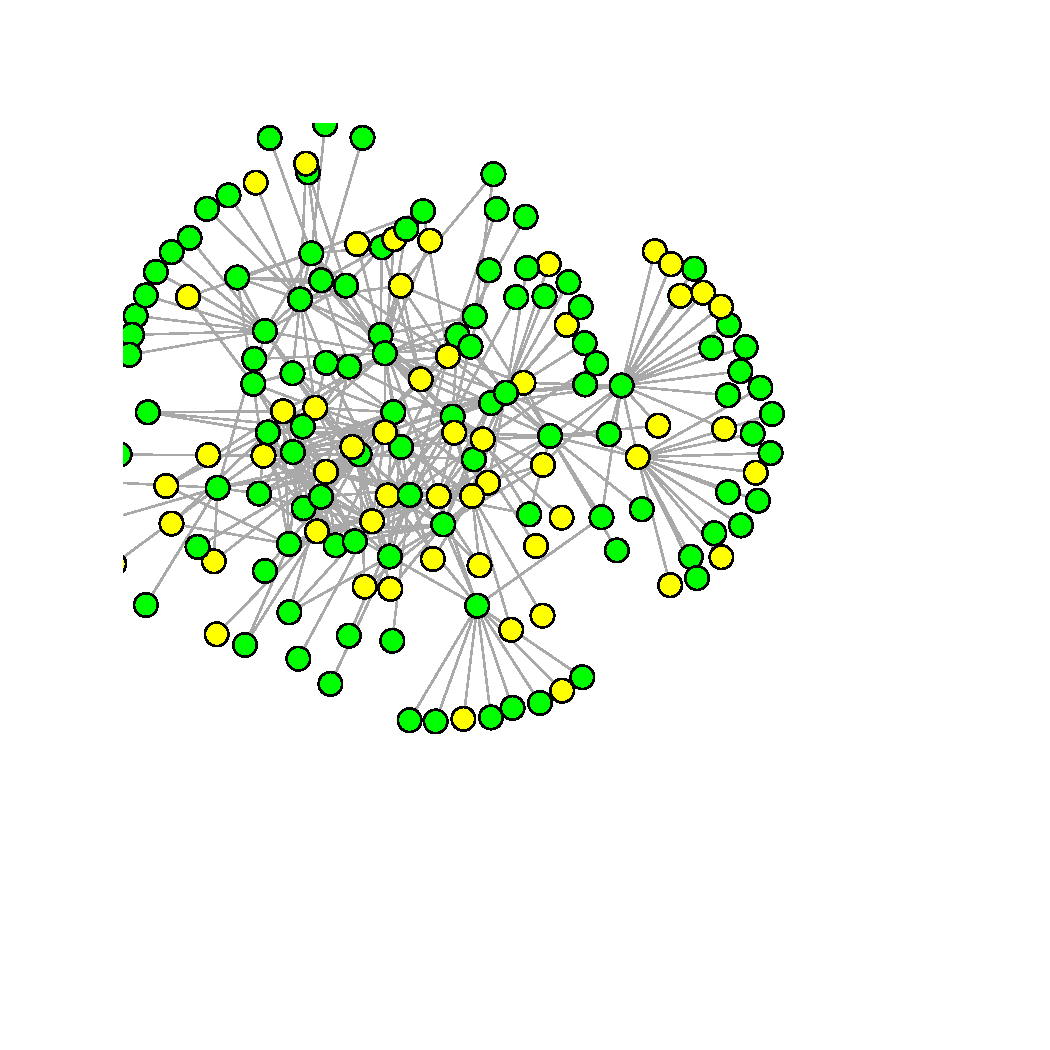
\includegraphics[width=0.5\textwidth,height=0.4\textheight]{"../results/figure2.png"}
\caption{Réseaux de collaborations des élèves du cours BIO500 à l'hiver
2022 avec et sans le cours TSB303. À gauche ont voit le réseau des
différentes collaborations sans celles provenant du cours TSB303 et à
droite le réseau de toutes les collaborations mais les liens mis en gras
représentent ceux du cours TSB303. les noeuds jaunes représente des
élèves n'étant pas en écologie alors que les noeuds vert sont des
étudiant en écologie.\label{fig:plot2}}
\end{figure}

La figure \ref{fig:plot3} est le réseau des différentes collaborations
depuis le début du baccalauréat entre les étudiants du cours de méthodes
en écologie computationnelle (BIO500) à l'hiver 2022 possédant 30
collaborations et plus. Dans cette situation, la modularité du réseau
est de 0.621.

\begin{figure}
\centering
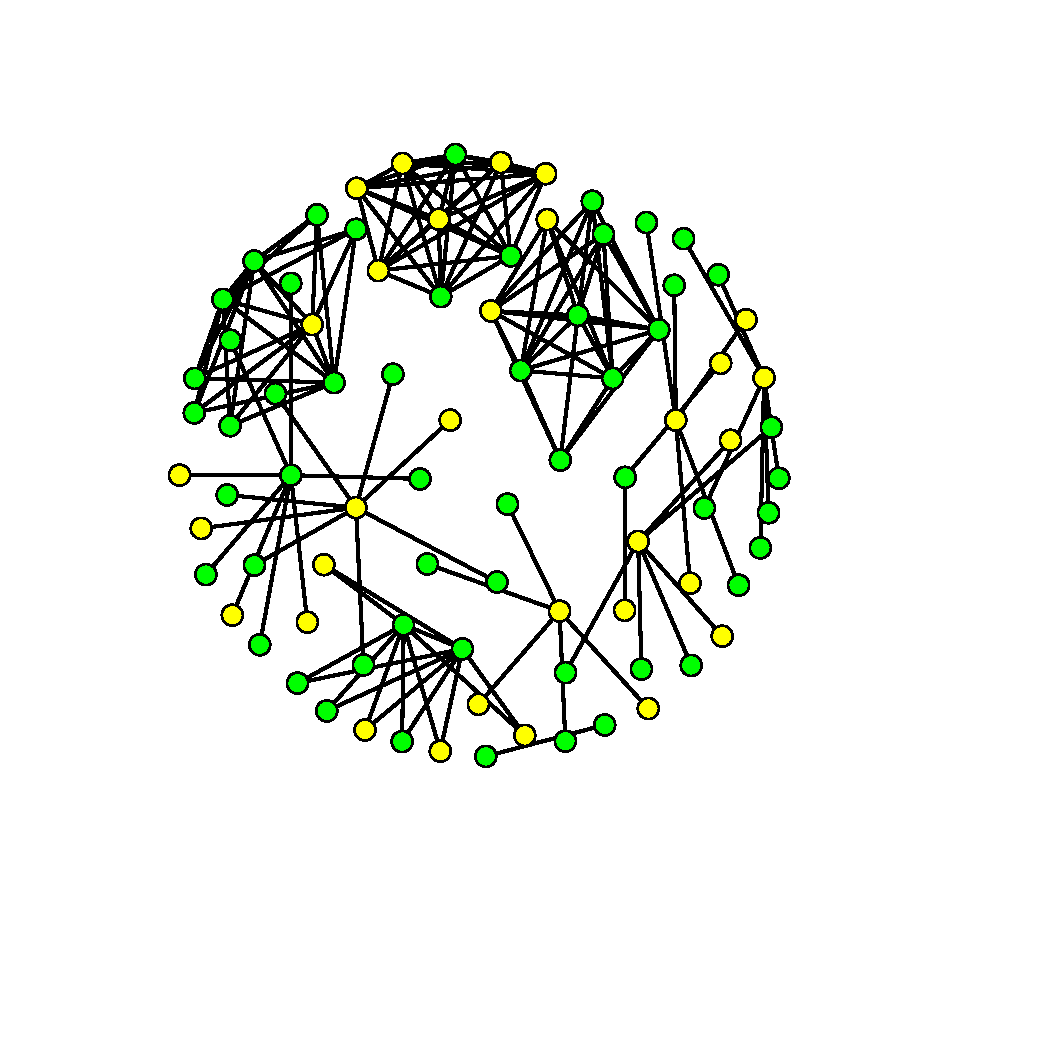
\includegraphics[width=0.5\textwidth,height=0.4\textheight]{"../results/figure3.png"}
\caption{Réseau de collaborations entre les élèves du cours BIO500 à
l'hiver 2022 qui ont plus de 30 collaborations. La grandeur et la
couleur des noeuds sont proportionnelles au nombre de collaborations de
chaque élève. La largeur des liens correspond au nombre de
collaborations entre la paire d'étudiant. \label{fig:plot3}}
\end{figure}

Notre quatrième et dernière figure (\ref{fig:plot4}) représente le
nombre d'étudiants pour différents nombres de collaborations (a) ainsi
que le nombre de collaborations différentes par étudiants (b),c'est à
dire le nombre de personnes distinctes avec qui ils ont coopérés pendant
le baccalauréat en écologie. C'est résultats sont aussi présentés sans
le cours TSB303 (c et d). La moyenne des collaborations différentes
entre étudiants est de 4.88 avec le cours TSB303 et de 4.83 sans le
cours TSB303.

\begin{figure}
\centering
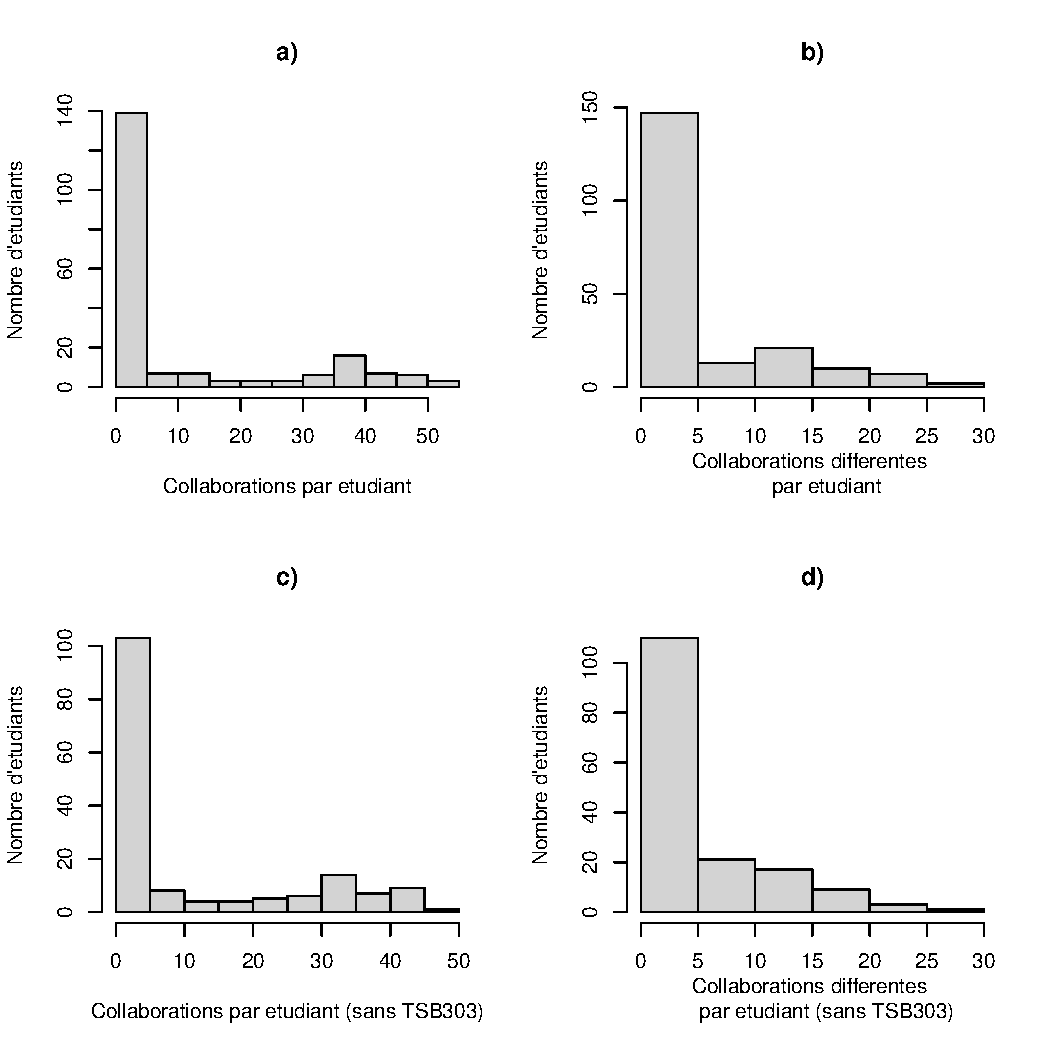
\includegraphics[width=0.5\textwidth,height=0.4\textheight]{"../results/figure4.png"}
\caption{Comparaison des collaborations totales et différentes des
élèves du cours BIO500 à l'hiver 2022 avec et sans le cours TSB303. (a)
Le nombre de collaborations par étudiant. (b) Le nombre de
collaborations différentes par étudiants. (c) Le nombre de
collaborations par étudiant snas TSB303. (d) Le nombre de collaborations
différentes par étudiant sans le cours TSB303. \label{fig:plot4}}
\end{figure}

\hypertarget{discussion}{%
\section{Discussion}\label{discussion}}

Rapidement, il est possible de remarquer que les élèves ont tendance à
utiliser le même réseau. Les cercles rapprochés les uns des autres
permettent de distinguer les élèves qui ont formé à plusieurs occasions
des groupes collaboratifs avec les mêmes étudiants afin d'accomplir
leurs travaux d'équipes durant leur baccalauréat. Une plus grande
diversité de collaborations aurait été visible s'il y avait eu une moins
grande ségrégation de groupes de cercles. Dans un tel cas, la figure
\ref{fig:plot1} tendrait vers une homogénéité et la grosseur des cercles
serait en moyenne plus importante.

Jugeant que 30 collaborations et plus correspondaient à un grand nombre
de collaborations, nous avons donc porté notre réflexion à comprendre ce
qui avait mené ces gens à obtenir autant de collaborations. Une méthode
couramment utilisée en écologie est le calcul du coefficient de Jaccard
(3) qui nous permettrait de quantifier l'hétérogénéité des interactions
par l'analyse des liens partagés. De cette manière, il serait possible
de distinguer des similarités dans la source du grand nombre de
collaborations de ces étudiants (4) et ainsi nous pourrions recommander
certaines directives aux professeurs afin d'augmenter le nombre de
collaborations des élèves.

Lorsqu'on ajoute le cours TSB303 aux collaborations, il avait été pensé
d'emblé que l'on verrait une augmentation du nombre de collaborations
apparaître. Essentiellement, la différence du nombre de collaborations
différentes avec ou le cours TSB303 n'est pas considérable. En revanche,
nous nous étions basé sur le fait que le nombre de collaboration pour ce
cours était de loin supérieur aux autres cours. Considérant, le fait
qu'un nombre important de gens semblent avoir oublié les collaborations
réalisées pour ce cours. Il serait fort probable que le cours TSB303
est, à lui seul, participer plus que les autres cours à augmenter le
nombre de collaborations différentes chez les élèves. Bien qu'il puisse
avoir eu un effet plus tangible sur le nombre différents de
collaborations. Nous ne pourrions pas recommander le type de
collaborations utilisé pour le cours TSB303. Le fait est que la quantité
ne semble pas toujours être la solution pour augmenter les bienfaits de
la collaboration. En effet, il faut également mentionner la qualité des
collaborations. Un travail de moins d'une dizaine de pages réalisé par
15 personnes ne laisse pas beaucoup de marge pour que le travail soit
réparti équitablement et donc la valeur du travail d'équipe peut être
amoindri. D'autant plus qu'à ce nombre de collaborations, le défi de
communication entre les membres de l'équipe est potentiellement plus
grand que l'accomplissement du travail lui-même. À terme, il semble donc
justifié de ne pas comparer ce type de collaboration aux autres où les
enjeux de collaborations ne sont tout simplement pas les mêmes.

\hypertarget{conclusion}{%
\section{Conclusion}\label{conclusion}}

Le réseau de collaboration nous démontre que le élèves du cours BIO500 à
l'hiver 2022 ont davantage été porté à conserver les mêmes
collaborations tout au long de leur parcours universitaire. Il serait
également possible d'approfondir nos connaissances sur la genèse d'un
grand nombre de collaborations via le calcul du coefficient de Jaccard
afin de pouvoir orienter les professeurs sur des pistes d'amélioration
en vu de former de meilleur futur travailleur. Tout en gardant en tête
que la qualité prévaut à la quantité des liens. Néanmoins, nous pouvons
d'ores et déja recommander aux professeurs d'être plus sensible à la
question, d'avoir un discours davantage porté à différencier les
collaborations et même peut-être à former eux-même les équipes afin
d'accentuer le nombre de collaborations différentes. Après tout c'est
eux qui forment les scientifiques de demain. Alors c'est à eux également
d'être plus alerte des lacunes systémiques.

\newpage

\hypertarget{bibliographie}{%
\section*{Bibliographie}\label{bibliographie}}
\addcontentsline{toc}{section}{Bibliographie}

\hypertarget{refs}{}
\begin{CSLReferences}{0}{0}
\leavevmode\hypertarget{ref-milgram1967small}{}%
\CSLLeftMargin{1. }
\CSLRightInline{Milgram S (1967) The small world problem.
\emph{Psychology today} 2(1):60--67.}

\leavevmode\hypertarget{ref-montoya2002small}{}%
\CSLLeftMargin{2. }
\CSLRightInline{Montoya JM, Solé RV (2002) Small {World} {Patterns} in
{Food} {Webs}. \emph{Journal of Theoretical Biology} 214(3):405--412.}

\leavevmode\hypertarget{ref-legendre2012numerical}{}%
\CSLLeftMargin{3. }
\CSLRightInline{Legendre P, Legendre L (2012) Numerical ecology, 3rd
english edition, v. 24.}

\leavevmode\hypertarget{ref-delmas2019analysing}{}%
\CSLLeftMargin{4. }
\CSLRightInline{Delmas E, et al. (2019) Analysing ecological networks of
species interactions. \emph{Biological Reviews} 94(1):16--36.}

\end{CSLReferences}



% Bibliography
% \bibliography{pnas-sample}

\end{document}
